\documentclass[a4paper, 12pt, twoside]{book}

\usepackage[utf8]{inputenc} %UTF8 codification
\usepackage[spanish]{babel} %spanish language compat
\usepackage{makeidx} %enable index creation
\usepackage[pass]{geometry} %change margins of a page
\usepackage{fancyhdr} %modify headers and footers
\usepackage[usenames,dvipsnames]{xcolor} %enable using colors 
\usepackage{graphicx} %include graphics
\usepackage{url} 
\usepackage{hyperref} %enable using pdf clickable url 
\usepackage{float} %for placing floating objecs like images
\usepackage{verbatim} %verbatim environment for writing
\usepackage{multirow} %multirow/column for tables
\usepackage{titlesec} %change titles styles
\usepackage{pbox} %paragraph box formatting text
\usepackage{listings, lstautogobble} %show code in boxes

\setlength{\marginparwidth}{0pt} %right margin width
\setlength{\parindent}{0pt} %no indent on the first line of a paragraph
\setlength{\parskip}{2mm} %space between paragraphs
\setcounter{tocdepth}{3} %depth of index (sections, subsetctions...)

\newcommand\anotacion[1]{\Large\textcolor{red}{\\#1\\}\normalsize} %Comamands for annotations
\newcommand\ant[1]{{\color{green}{#1}}}
\includeonly{summary, abstract, introduction, waveMigration, androidApp, results, futureWork, ref, append} %include archives

%\renewcommand{\chaptername}{}
%\renewcommand{\thechapter}{}

%% Redefine the style for the cover
\fancypagestyle{cover}
{
   \fancyhf{} % delete the current heading/footer configuration
   \lfoot{
\includegraphics[keepaspectratio, scale=0.8]{Media/cc.png}} %include image on left foote
   \renewcommand{\headrulewidth}{0pt}
}

%% Redefine the style for the pages with section
\fancypagestyle{sectioned}
{
   \fancyhf{}
   \rhead{} %right header content
   \renewcommand{\headrulewidth}{0pt} %size of the separator line of header
}

% define style for console commands
\lstdefinestyle{console}
{
breaklines=true, 
autogobble=true, 
basicstyle=\ttfamily\footnotesize,
backgroundcolor=\color{gray!70},
}

\makeindex %create index


\titleformat{\chapter}[display] %formating chapter title format 
{\normalfont\huge\bfseries}{\chaptertitlename\ \thechapter}{20pt}{\Huge}
\titlespacing*{\chapter}{0pt}{0pt}{30pt} %formating chapter title spacing [left, beforeVertical, afterVertical] 

\begin{document}

%% Front page
\pagestyle{fancy}
\renewcommand{\headrulewidth}{0pt}
\fancyhf{}
\cfoot{\fancyplain{}{\thepage}} %show the number of page on footer center
\lhead{}
\newgeometry{margin=2.5cm} %redefine margins
\begin{titlepage}
\pagenumbering{Roman}
\setcounter{page}{1}

\newpage
\thispagestyle{cover}
\begin{center}
  {\Huge \bf \textit{DemoCritics}} \\
  \vspace*{0.5cm}
  {\large \bf Aplicación Android de participación política con edición colaborativa en tiempo real}

  \vfill
  {\LARGE\bf Jaime Ramos Romero\\
    \vspace*{0.5cm}
	     Javier Bastarrica Lacalle}

  \vfill

  {\Large\bf Grado en Ingeniería Informática\\}
  {\Large\bf Facultad de Informática\\}
  \vspace*{0.4cm}
  {UNIVERSIDAD COMPLUTENSE DE MADRID}
  \vspace*{0.8cm}
  
   \begin{center}
   
\includegraphics[keepaspectratio, scale=0.12]{Media/ucmlogo.png}
   \end{center}
  
  \vspace*{0.5cm}

  {\large\bf Trabajo de Fin de Grado\\
             Madrid, Junio 2015\\}
  \vspace*{0.7cm}
  {\large Directores:\\
          Samer Hassan Collado\\
          Pablo Ojanguren}
  \vfill

  \rhead{}
  \rfoot{}
  \fancyhf{}

\end{center}
\end{titlepage}
\restoregeometry


\addtocontents{toc}{~\hfill\textbf{Page}\par}

%%%%%%%%%%%%%%%%%%%%%%%%%%%%%%%%%%%%%%%%%%%%%%%%%%%%%%%%%%%%%%%%%%%%%%%%%%%
%%%%%%%%%%%%%%%%%%%% Authorization of dissemination %%%%%%%%%%%%%%%%%%%%%%%  
%%%%%%%%%%%%%%%%%%%%%%%%%%%%%%%%%%%%%%%%%%%%%%%%%%%%%%%%%%%%%%%%%%%%%%%%%%%
\newpage
\thispagestyle{empty}
%\addcontentsline{toc}{chapter*}{\numberline{}Authorization of dissemination
%                                            and usage}
\chapter*{Autorización de Difusión y Uso}
\addcontentsline{toc}{chapter}{\numberline{}Autorización de Difusión y Uso}
%\begin{center}
%  \textbf{\Huge Authorization of dissemination and usage}
%\end{center}
\vfill
Autorizo a la Universidad Complutense de Madrid a difundir y utilizar con fines académicos, no comerciales y mencionando expresamente a su autor, tanto la propia memoria, como el código, la documentación y/o el software desarrollado. 
\begin{center}
  \vfill
  {\Large Jaime Ramos Romero\\
	  Javier Bastarrica Lacalle\\}
  \vspace*{4cm}
  {\Large Madrid, Junio 2015}
  \vfill
\end{center}
  Copyleft by Jaime Ramos Romero and Javier Bastarrica Lacalle, released under the license Creative Commons Attribution Share-Alike International 4.0 available at:
\begin{center}
\url{https://creativecommons.org/licenses/by-sa/4.0/}
\end{center}

%%%%%%%%%%%%%%%%%%%%%%%%%%%%%%%%%%%%%%%%%%%%%%%%%%%%%%%%%%%%%%%%%%%%%%%%%%%
%%%%%%%%%%%%%%%%%%%%%%%%%%% Acknowledgements %%%%%%%%%%%%%%%%%%%%%%%%%%%%%%
%%%%%%%%%%%%%%%%%%%%%%%%%%%%%%%%%%%%%%%%%%%%%%%%%%%%%%%%%%%%%%%%%%%%%%%%%%%

\newpage
\thispagestyle{empty}

\chapter*{Agradecimientos}
\addcontentsline{toc}{chapter}{\numberline{}Agradecimientos}

Agradezco...


%%%%%%%%%%%%%%%%%%%%%%%%%%%%%%%%%%%%%%%%%%%%%%%%%%%%%%%%%%%%%%%%%%%%%%%%%%%
%%%%%%%%%%%%%%%%%%%%%%%%%%% Tables of contents %%%%%%%%%%%%%%%%%%%%%%%%%%%%
%%%%%%%%%%%%%%%%%%%%%%%%%%%%%%%%%%%%%%%%%%%%%%%%%%%%%%%%%%%%%%%%%%%%%%%%%%%
\newpage
\tableofcontents
%\let\clearpage\relax
\newpage
\setcounter{page}{7}
{\listoffigures \let\cleardoublepage\relax \listoftables}
%\listoffigures
%\listoftables
\newpage


%% Main text
% set page number starts from 1
\pagenumbering{arabic}

\newpage
\renewcommand{\thepage}{\Roman{page}}
\setcounter{page}{9}
\chapter*{Abstract}
\addcontentsline{toc}{chapter}{\numberline{}Abstract}
Nowadays we live in a society of democratic change in which people begin to take a decisive role  in the political area. There are increasingly social movements that proliferate due to the interest generated by taking part in politics. This participation has been channeled by the emergence of new technologies that allows to establish new ways for people to organize and express their opinion. The vast majority of these new tools are developed in a scope near to Web-based interfaces and interconnected network platforms. Being as we are in a time subject to several electoral events that favours the increased interest of people involved in politics, the development of such type of tools is becoming increasingly necessary.

Keeping in mind this context, we contemplate the development of an application that provides access to new ways of participation from mobile devices. This application will have two clear objectives: to bring to the forefront political programmes, which usually few people read, encouraging its reading and discussion; and open a common space in which citizens express their alternative proposals to those put forward by the political parties that represent us.
 
We will base on the use of already existing Open-Source technologies for collaborative editing in real-time, adjusting them to mobile devices. Specifically we will explore the use of Web-based platform Apache Wave, carrying out a migration process that allows to take advantage of its potential in Android-based devices. This migration supposes an additional work that involves an effort to research into the development of an innovative platform, because there is no equivalent free software currently on Android. By using this technology, users will have the opportunity to compose real-time collaborative texts.

As a result for this work we will develop a first version of the application which, as a proof of concept, will make use of the features described above. Thus, the ultimate aim we set out for this project is to put into practice its usefulness during future electoral events.
\vfill
{\large \bf Keywords:}\\
{\large Collaborative Writing, Politics, Democracy, Citizen Participation, Real-Time, Android, Apache Wave, Elections, Election Programme, Citizen Proposals. }

\newpage
\renewcommand{\thepage}{\Roman{page}}
\setcounter{page}{10}
\chapter*{Resumen}
\addcontentsline{toc}{chapter}{\numberline{}Resumen}
Actualmente vivimos en una sociedad de cambio democrático en la que las personas comienzan a adquirir un papel determinante en el terreno político. Son cada vez más los movimientos sociales que proliferan a raíz del interés generado por participar en politica. Esta participación se ha visto canalizada por la aparición de nuevas tecnologías que permiten establecer nuevas formas para que las personas se organicen y expresen su opinión. La gran mayoría de estas nuevas herramientas se desarrollan en un ámbito cercano a plataformas interconectadas en red y basadas en una interfaz Web. Encontrándonos en un momento sujeto a varias citas electorales que propicia el aumento del interés de las personas por involucrarse en política, el desarrollo de este tipo de herramientas se hace cada vez más necesario.

Teniendo en cuenta este contexto, se plantea el desarrollo de una aplicación que proporcione acceso a nuevas formas de participación desde dispositivos móviles. Dicha aplicación tendrá dos objetivos claros: poner en un primer plano los programas electorales (que normalmente pocas personas leen) incentivando su lectura y debate; y abrir un espacio común en el que la ciudadanía exprese sus propuestas alternativas a las soluciones expuestas por los partidos políticos que les representan.

Nos basaremos en el uso de tecnologías de Software libre ya existentes de edición colaborativa en tiempo real, adaptándolas a dispositivos móviles. Concretamente se explorará el uso de la plataforma Web Apache Wave, llevando a cabo un proceso de migración que permita explotar su potencial en dispositivos basados en Android. Esta migración supone un trabajo adicional que conlleva un esfuerzo de investigación y desarrollo de una plataforma innovadora, ya que no existe una tecnología de software libre equivalente en Android actualmente. Haciendo uso de esta tecnología los usuarios tendrán la oportunidad de redactar textos colaborativos en tiempo real.

Como resultado de este trabajo se desarrollará una primera versión de la aplicación que, a modo de prueba de concepto, haga uso de las funcionalidades antes descritas. De esta manera el objetivo final que nos planteamos es poner en práctica su uso durante futuras citas electorales.

\vfill
{\bf Palabras Clave:}\\
{Escritura Colaborativa, Política, Democracia, Participación Ciudadana, Real-Time, Android, Apache Wave, Elecciones, Programas Electorales, Propuestas Ciudadanas.}

\newpage
\thispagestyle{empty}
\mbox{}



\pagestyle{fancy}
\renewcommand{\headrulewidth}{1pt}
%\renewcommand{\sectionmark}[1]{\markright{#1}}
\fancyhf{}
\rhead{\MakeUppercase{\leftmark}}
\cfoot{\fancyplain{}{\thepage}}
\lhead{}

\newpage
\thispagestyle{sectioned}
\pagenumbering{arabic}
\chapter{Introducción}

A continuación se exponen de forma resumida los objetivos que se persiguen al realizar este Trabajo de Fin de Grado y un esquema de la estructura de esta Memoria.

ANTECEDENTES Y ALARGAR

\section{Marco teórico de la idea: Política en el mundo de la Informática}

En los siguientes párrafos se discutirá acerca de una serie de consideraciones sobre el estado actual de la política y la democracia. Se centrará sobre todo en su relación con las nuevas tecnologías como herramientas capaces de cambiar la manera en la que se conciben ambas disciplinas.

A primera vista se puede pensar que la política no parece entusiasmar a las personas dedicadas al mundo de la informática. Se puede ubicar la política como una parte de las ciencias sociales o la actividad política, situando la informática en ciencias exactas o formales. Pero pensando en factores como la gestión de los privilegios de una aplicación entre los que se define de alguna forma una jerarquía, indirectamente se estará haciendo política. También se pueden encontrar características políticas en el diseño relacional de una base de datos. Definiendo los campos de una base de datos se pueden ver algunos valores como el sexo, la nacionalidad, la edad o incluso las relaciones o restricciones que existen entre las tablas. Se estarán definiendo unas reglas básicas de funcionamiento de la base de datos establecidas por unos principios políticos.

Adentrándose en el mundo de las Licencias (copia, modificación, distribución, etcétera) en el desarrollo de \textit{Software} se encuentra más contenido político. Licencias que determinan el uso de un tipo de \textit{Software}, ya sea para compartir, vender o distribuir copias. Multitud de ''reglas políticas'' definidas en un documento de licencia de uso. Así como las restricciones que se establecen en la metodología del desarrollo orientado a objetos, estableciendo las relaciones de herencia, restricción de métodos, variables, etcétera.

Regresando a la actualidad y basándose en no muy lejanos acontecimientos pasados, se ha oído cómo algunos gobiernos recopilan datos de la actividad de los usuarios en las redes sociales \cite{ref:NSAData}, analizando todo el contenido que generan. Incluso cómo algunas aplicaciones móviles piden aprobar permisos con los que operar libremente en los dispositivos.

Se observa por tanto que la política está más integrada en la informática de lo que parece, sobre todo si se deja a un lado la informática más científica y formal y se pasa a la informática más social, la de los gobiernos, la de los negocios o la de las relaciones sociales.

\section{Adentrándonos en la idea}

La idea a desarrollar está generada en una época en la que la política parece haber despertado el interés de una parte considerable de la ciudadanía. Podría ser por tanto una herramienta útil para participar en temas políticos de forma sencilla y atractiva. Dejando así atrás los tópicos a menudo escuchados de \textit{"yo no entiendo de política"}, \textit{"la política es aburrida"}, \textit{"no sé a quién votar"} o \textit{"no he leído nunca un programa electoral"} entre otros.

La herramienta ofrecería una nueva forma de participar en la política y de llevar a los ciudadanos los programas electorales expuestos por las diferentes formaciones políticas. De forma que, para potenciar el uso social de la aplicación, los ciudadanos podrían leer aquellos puntos de los programas más vistos, debatidos, comentados, etc. Así, cualquier usuario tendría a su disposición todos los programas electorales en su bolsillo, por lo que no tendría que ir a la página web de cada formación política y descargarse un documento de 200 páginas. Pensamos que esta forma tradicional de presentar un programa político en un solo documento en un mundo donde las posibilidades de comunicarnos se han desarrollado exponencialmente mediante las nuevas tecnologías no es la mejor manera de generar interés por su lectura y la implicación en política de las personas.

Por otra parte, y teniendo en cuenta la tendencia actual de los nuevos movimientos ciudadanos de elaborar programas políticos en base a propuestas de los ciudadanos, \textbf{la aplicación también debía ofrecer alguna manera de realizar Propuestas y debatirlas entre todos}. De esta forma tanto la ciudadanía como las formaciones políticas podrían saber en cualquier momento cuáles son las principales preocupaciones de los ciudadanos y qué medidas o soluciones proponen para resolverlas. \textbf{Además pensamos que podríamos aprovechar las características de Wave para realizar estas Propuestas de forma colaborativa y en tiempo real}, aportando un valor diferenciador respecto a las actuales soluciones desarrolladas para web (Ver sección \ref{ssec:artProposals}).

Por tanto, desde un primer punto de vista subjetivo, la aplicación quedó dividida en dos partes. Por un lado tendríamos la presentación estructurada de los programas políticos que presentan las formaciones políticas. Y por otro todas las propuestas que elaboran de forma colaborativa los ciudadanos, ya sea individualmente o en colectivos sociales.
 
 
\section{Objetivos del Proyecto}

El objetivo principal de este proyecto es desarrollar una aplicación Android de utilidad social y que haga uso de una tecnología poco usada en estas plataformas móviles como es la colaboración en tiempo real, que desde hace unos años sí que viene estando más presente en plataformas Web. Para ello primero se evaluará la tecnología existente en el proyecto SwellRT (basado en Apache Wave) y se adaptará dicha tecnología para poder hacer uso de ella de forma nativa desde Android. Después se discutirán posibles ideas de aplicación que puedan hacer uso de esta tecnología y se diseñará y desarrollará una primera versión estable de esa idea de aplicación Android que pueda ser evaluable por usuarios. También se estudiará la viabilidad de seguir desarrollando a futuro la aplicación con vistas a conseguir un producto que podamos poner a disposición del público en el \textit{marketplace} de Android.

\begin{itemize}
  \item {
    1ª parte: Migración de Wave (SwellRT) a Android
    \begin{itemize}
      \item Proporcionar un entorno de colaboración en tiempo real federado para Android basado en SwellRT.
    \end{itemize}
  }
  \item {
    2ª parte: Creación de la aplicación Android.
    \begin{itemize}
      \item Desarrollar una aplicación que recopile y permita interactuar con los programas electorales de los partidos políticos.
      \item Desarrollar una aplicación que permita la participación colectiva de ciudadanos mediante propuestas colaborativas editables en tiempo real.
    \end{itemize}
  }
\end{itemize}

\section{Estructura del Documento}

En esta memoria se han querido reflejar los aspectos más destacados del proceso de desarrollo de este Trabajo de Fin de Grado. Aunque a lo largo del documento se detallen aspectos técnicos queremos dejar patente que no se trata de un tutorial de cómo funciona Wave o Android. Aunque a veces se entre en mayor detalle por cuestiones de claridad a la hora de entender el funcionamiento de la tecnología, se anima al lector si quiere profundizar más en el tema a que haga uso de las múltiples referencias bibliográficas que se incluyen en este documento.  

A lo largo de este documento el lector se encontrará con una estructura basada en capítulos en los que se irán detallando distintas facetas del desarrollo del proyecto: 

\begin{itemize}
  \item \textbf{Capítulo 2 - Construyendo la idea de la aplicación DemoCritics:} se expone cómo y por qué se llegó a la idea de esta aplicación tras haber realizado la migración de SwellRT a Android.
  \item \textbf{Capítulo 3 - Estado del Arte:} se hace un pequeño análisis de las características de actuales soluciones software que hacen uso de tecnologías de colaboración en tiempo real y de aplicaciones dedicadas a la participación política.
  \item \textbf{Capítulo 4 - Tecnologías del Proyecto:} se repasan las tecnologías y herramientas utilizadas durante todo el desarrollo del proyecto.
  \item \textbf{Capítulo 5 - Metodologías del Proyecto:} se detallan el proceso de migración de SwellRT y metodologías utilizadas el diseño, implementación y evaluación de DemoCritics.
  \item \textbf{Capítulo 6 - Arquitectura del Proyecto:} se indaga en aspectos técnicos destacados de la organización de DemoCritics.
  \item \textbf{Capítulo 7 - Resultados, Conclusiones y Trabajo Futuro:} se discuten los resultados obtenidos con el objeto de sacar algunas conclusiones. Se discuten los siguientes pasos a realizar con el objetivo  de mejorar o cambiar DemoCritics.
\end{itemize}

\newpage
\thispagestyle{sectioned}
\chapter{Migración de Wave a Android}

\section{Estado del Arte}

 ---- PENDIENTE ----

\section{Wave}
  
  \subsection{Google Wave}

  Ideado y presentado en 2009 por ingenieros de Google \cite{ref:wave_announcement}, Wave es a la vez un protocolo de comunicaciones \cite{ref:wave_over_xmpp} y una plataforma web de código libre, que permiten a sus usuarios comunicarse y colaborar entre sí en tiempo real (Ver sección \ref{sssec:realTime}) y de forma federada (Ver sección \ref{sssec:federation}) a través de Internet. 
  Inicialmente fue desarrollado con el objetivo de integrar en una sola plataforma servicios ampliamente utilizados como son el correo electrónico, las redes sociales y la mensajería instantánea. Pese al gran entusiasmo generado entre la comunidad de desarrolladores tras su anuncio, en el año 2010 Google anuncia el abandono del proyecto \cite{ref:google_wave_end} debido a su poca acogida entre los desarrolladores y a que decide reorientar el uso de la tecnología hacia sus plataformas de edición de documentos Google Docs \cite{ref:google_docs} y a su red social Google + \cite{ref:google_plus}.  Es en este momento cuando el desarrollo libre del proyecto pasa a manos de la Apache Software Foundation bajo el nombre de Apache Wave.

  \subsection{Apache Wave}
  
  Al cambiar de manos su desarrollo en 2010, la tecnología pasa a formar parte de la incubadora de la fundación Apache \cite{ref:apache_wave_about} como software de código libre bajo licencia Apache \cite{ref:apache_license}. Así, se produce el desarrollo de Wave In a Box (WIAB) (Ver sección \ref{sec:wiab}), plataforma que integra un cliente web sencillo y una implementación de un servidor Wave que cualquiera puede descargar y desplegar en su ordenador.   

\section{Tecnologias y Caracteristicas de Wave}
  
  \subsection{Caracteristicas de Wave}
  
  Como plataforma de código libre desarrollada para ser utilizada en red, Wave hace uso de distintas tecnologías y protocolos bien conocidos. Entre sus características más destacadas están las siguientes:

    \subsubsection{Federación}\label{sssec:federation}
    
    El Protocolo Wave \cite{ref:wave_over_xmpp} fue desarrollado para utilizar un modelo federado \cite{ref:wave_federation} \cite{ref:wave_white_paper} de comunicación basado en la tecnología XMPP \cite{ref:xmpp} \cite{ref:wave_over_xmpp}. Se trata por tanto de un modelo descentralizado en el que cualquiera de los participantes en la conversación es libre de actuar tanto como servidor como cliente sin que ello afecte a su participación en la conversación. 
    Además, a diferencia de otras tecnologías (como el correo electronico) en las que cada participante almacena su propia copia de la conversación y cada vez que hay cambios se debe transmitir la conversación entera a todos los participantes, Wave tiene la ventaja de que actúa de forma que es el servidor de la conversación el único que almacena la copia entera y se encarga de calcular los cambios que se han producido para transmitir solamente dichos cambios por la red a los participantes, con las consiguientes ventajas en términos de latencia que ello conlleva. 

    \subsubsection{Consistencia en tiempo real}\label{sssec:realTime}
    
    El Protocolo Wave \cite{ref:wave_over_xmpp} utiliza la tecnología de Transformaciones Operacionales (OT) \cite{ref:how_ot_works} para garantizar la consistencia en la comunicación en tiempo real entre los participantes. Es decir, cualquier cambio producido por cualquiera de los participantes en la conversación se transmite automáticamente y en tiempo real al resto de los participantes sin pérdida de información y garantizando que los cambios se muestran en el estricto orden en el que se produjeron sin errores \cite{ref:wave_ot}.
    
    \subsubsection{Escalabilidad}
    
    Wave fue desarrollado como un protocolo de alta escalabilidad que permite gestionar la existencia de una gran cantidad de conversaciones y participantes sin que por ello se resienta la productividad del sistema.
    
    \subsubsection{Modelo Wave}\label{sec:waveModel}
    
    Además de definir el protocolo del que hace uso Wave, Google definió un Modelo de Datos Conversacional \cite{ref:wave_conversation_model} que refleja la arquitectura de los datos que componen las conversaciones en Wave. Así, a grandes rasgos, podemos ver dichas conversaciones como documentos XML sobre los que los usuarios participantes (cualquiera es libre de unirse a una conversación en cualquier momento) actúan creando nuevos elementos o modificando los ya existentes. Este modelo de datos define una nomenclatura propia para los elementos que componen esta tecnología \cite{ref:wave_api_overview} \cite{ref:wave_white_paper}:
    
      \begin{itemize}
	\item \textbf{Wave}: Conjunto de wavelets (conversaciones).
	\item \textbf{Wavelet}: conjunto de documentos de una conversación y sus participantes.
	\item \textbf{Blip}: documento con el contenido de un mensaje en la conversación. Un blip puede tener otros blips dentro de él y los blips pueden ser publicados o no en función de si su visibilidad se extiende o no al resto de participantes de la conversación respectivamente.
	\item \textbf{Manifiesto conversacional}: documento con metadatos que definen la estructura de una conversación. 
	\item \textbf{Hilo conversacional}: conjunto de Blips consecutivos que forman parte de una conversación.
	\item \textbf{Extensiones} \cite{ref:wave_extensions}: pequeñas aplicaciones que se ejecutan dentro de una Wave y aportan nuevas funcionalidades que no forman parte del modelo conversacional básico. Pueden ser de dos tipos:
	  \begin{itemize}
	    \item \textbf{Gadget}: aplicación que se ejecuta en el contexto de una Wave y en la que todos sus usuarios participan.
	    \item \textbf{Robot}: aplicación que participa en una Wave a modo de usuario automatizado e interactúa con el contenido pudiendo modificarlo y responder a eventos por acciones de otros usuarios reales.
	  \end{itemize}
      \end{itemize}
      
       \begin{figure}[H]
	  \centering
	    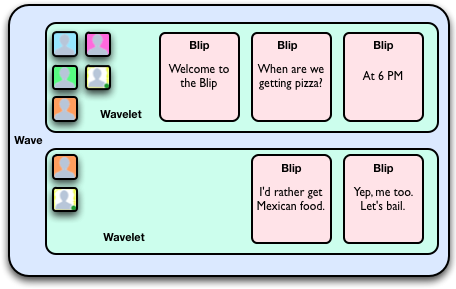
\includegraphics[keepaspectratio, scale=0.8]{Media/Captures/waveEntities.png}
	  \caption{Modelo Conversacional de Wave}
	  \label{fig:wave_model}
	\end{figure}
  
  \subsection{Servidores Wave}
  
    \subsubsection{Wave in a Box}\label{sssec:wiab}
    
    Wave In a Box (WIAB) \cite{ref:wave_in_a_box} es el nombre de la implementación de un servidor Wave desarrollado por la Apache Software Foundation tras pasar el proyecto a sus manos en el año 2012. Al igual que el resto del código de la tecnología que heredó de Google, está implementado en Java usando OpenJDK \cite{ref:openjdk}. La instalación trae consigo un cliente web desarrollado en Javascript usando el framework Google Web Toolkit \cite{ref:gwt}. Este cliente web sirve como prueba de concepto de las funcionalidades básicas del Modelo Conversacional de Wave, pudiendo gesionar waves, usuarios y extesiones. Actualmente cualquiera puede descargar y desplegar WIAB en su ordenador siguiendo los pasos que nos proporcionan en su wiki \cite{ref:wave_in_a_box_wiki}. La aplicación se distribuye en forma de código fuente, accesible entre otras formas desde su repositorio de GitHub \cite{ref:wave_in_a_box_github}. Existen asimismo servidores de prueba ya desplegados en Internet sobre los que se puede observar el funcionamiento de WIAB \cite{ref:wave_in_a_box_server}.
   
   
    \begin{figure}[H]
      \centering
	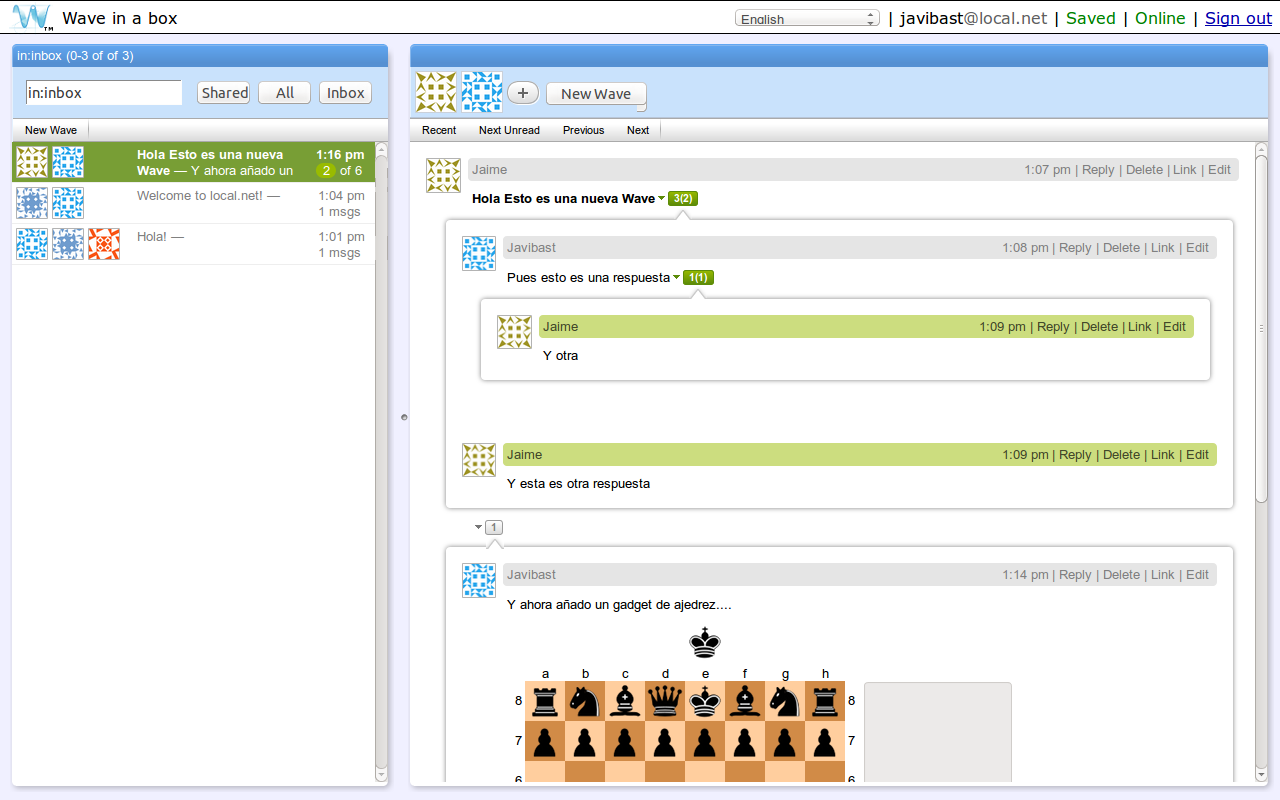
\includegraphics[keepaspectratio, scale=0.3]{Media/Captures/WIAB_Server.png}
      \caption{Cliente Wave In A Box}
      \label{fig:wiab_client}
    \end{figure}
   
    \subsubsection{SwellRT}
    
    Como parte del proyecto europeo P2PValue \cite{ref:p2pvalue} existe SwellRT, un fork de WIAB que amplía las características de éste último añadiendo un nuevo modelo de datos (Modelo de Datos Colaborativo) más allá del Modelo de Datos Conversacional de Wave original. Proporciona también un API escrito en Java que permite trabajar sobre los datos de ese nuevo modelo en forma de tres tipos básicos: mapas, listas y strings. Es por tanto un framework de colaboración en tiempo real que basa su funcionamiento en Apache Wave y cuyo principal popósito es permitir la integracion de la tecnología Wave en otras aplicaciones, que podrán compartir objetos (de los tipos antes mencionados) de forma federada y en tiempo real. Su código fuente está disponible en GitHub \cite{ref:swellRT_github}, así como sus instrucciones de instalación (Ver el Readme en GitHub).\\[.2cm]

    Para este proyecto se ha usado el framework SwellRT como base para la migración de la tecnología de Apache Wave a la plataforma Android \cite{ref:android_platform}. Se pretende con esto que SwellRT haga uso de las funcionalidades nativas de Android.

  
\section{Metodología de Migración}
  
  \subsection{Objetivo}
  
    El framework de SwellRT utiliza un servidor WIAB y el protocolo Wave, ambos desarrollados en Java. El \textbf{SDK de Android} \cite{ref:android_sdk} es compatible con Java, así que a priori la implantación del servidor no supone problemas en los dispositivos móviles. Sin embargo, existe un problema con el API de SwellRT, ya que el lado del cliente fue desarrollado en Javascript usando el framework GWT. Android no soporta de forma nativa estas tecnologías, así que es necesario estudiar el código de SwellRT para sustituir todo el código que haga uso de Javascript/GWT por código compatible con Android. El objetivo de esta parte del proyecto es conseguir que un cliente desplegado en Android sea capaz de conectarse e interactuar con un servidor Wave sin problemas.  
  
  \subsection{Plataforma: Entorno de Desarrollo, Construcción y Depuración}
  
    Existen dos entornos de desarrollo (IDE) recomendados por Google para desarrollar en Android: Eclipse \cite{ref:eclipse} y Android Studio.\cite{ref:android_studio} Eclipse es un entorno de desarrollo genérico que, mediante plugins, permite extender sus funcionalidades para desarrollar en diversas plataformas y lenguajes. Android Studio es un IDE basado en el entorno de desarrollo Java IntelliJ IDEA \cite{ref:intelliJ_Idea} adaptado para trabajar con todas las funcionalidades de Android. En el momento de empezar con la migración Android Studio se encuentra en fase beta de desarrollo, pues Google pretende convertirla en el IDE de desarrollo oficial para Android. Mientras no se lanza la version final de Android Studio, Google recomienda utilizar Eclipse para desarrollar en Android, y las guias para desarrolladores Android estan escritas para Eclipse. En consecuencia tomamos la decision de utilizar el entorno de desarrollo Eclipse para la migracion de SwellRT a Android. 

    \subsubsection{Eclipse} \label{sssec:eclipse}
    
    El IDE de Eclipse \cite{ref:eclipse} soporta el desarrollo con Android a través del plugin \textbf{ADT (Android Development Tools)} \cite{ref:eclipse_adt}, que integra en un solo paquete todas las herramientas necesarias para desarrollar, construir y depurar el código de la aplicacion fácilmente. \\[.2cm]
    
    \textbf{Android SDK} \cite{ref:android_sdk}: paquete que integra el conjunto de herramientas necesarias para desarrollar en Android.  Entre estas herramientas destacan las siguientes:
    
    \begin{itemize}
    \item \textbf{Librerías con el API} de Android y \textbf{Documentación} asociada \cite{ref:android_api_reference}
    
    \item \textbf{Android Virtual Device Manager (AVDM)} \cite{ref:android_vdm} herramienta para gestionar la creación, modificación, ejecución y eliminación de emuladores en Android. Un \textbf{emulador} \cite{ref:android_emulator} es una máquina virtual que ejecuta una determinada versión de Android. Permite desplegar un dispositivo movil en el ordenador que imita las características software y hardware de uno real para poder hacer pruebas de desarrollo sin necesidad de poseer un dispositivo con Android. 
    
    \item \textbf{Android SDK Manager} \cite{ref:android_sdk_manager} herramienta para gestionar las versiones de SDK y herramientas asociadas instaladas. Android se encuentra actualmente en la versión 5.1 (API 22), pero un desarrollador puede elegir desarrollar para una versión anterior si lo estima necesario, por lo que puede descargarse por separado dicha versión y mantener varias API si lo necesita.
    
    \item \textbf{Dalvik Debug Monitor Server (DDMS)} \cite{ref:android_ddms} herramienta que provee las características de entorno de depuración para las aplicaciones en desarrollo.

    \end{itemize}
	
	Teniendo en cuenta la distribucion actual de versiones instaladas en dispositivos Android \cite{ref:android_dist} (Ver figura \ref{fig:android_Usage}) se ha decidido realizar la migración de SwellRT con el API 19 de Android (Version 4.4 "KitKat"). El emulador desplegado para las pruebas de desarrollo utilizará por tanto Android 4.4 .

	\begin{figure}[H]
      \centering
	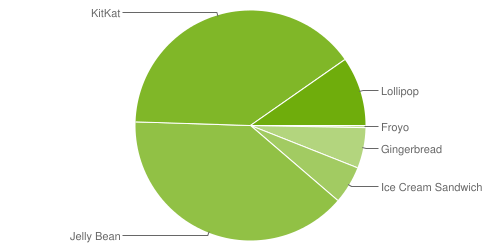
\includegraphics[keepaspectratio, scale=0.8]{Media/Captures/androidUsage.png}
      \caption{Distribución Actual de Versiones Android (Fuente: Google)}
      \label{fig:android_Usage}
    \end{figure}

	Sin embargo existe un problema con la construcción y depuración del código de SwellRT en Eclipse. Android \textbf{limita el número de métodos máximos de una aplicacion a 65K} \cite{ref:android_limit65k} por cuestiones de eficiencia. Para evitar esta limitación, durante el proceso de construcción el SDK de Android utiliza, entre otras, una herramienta llamada \textbf{ProGuard} \cite{ref:android_proguard}. Esta herramienta se encarga de optimizar el código de la aplicacion buscando remover clases que no se utilizan y ofuscando el código para prevenir la ingeniería inversa. En el caso de SwellRT, el código posee un gran número de clases java necesarias para desplegar el servidor y el cliente de la herramienta, por lo que es necesaria dicha optimización de código realizada por ProGuard. El sistema de compilación de aplicaciones de Android tiene dos formas: compilacion de la aplicacion en modo debug (para hacer pruebas cuando todavía se encuentra en fase de desarrollo) y en modo release (la aplicación se encuentra en su versión final y se empaqueta y se firma digitalmente para lanzarla al público). En el caso de Eclipse, ProGuard solo se ejecuta cuando se construye en modo release, por lo que cuando se intenta compilar una aplicación con tantas clases como SwellRT mientras se desarrolla (modo debug) el sistema da error y no se puede compilar el código para probarlo en el emulador. \\[.2cm]

	La solución que encontramos fue desarrollar en Eclipse (por las facilidades que el entorno proporciona para escribir código) pero realizar el proceso de construcción del código por consola de comandos, ya que en este caso sí que se puede compilar la aplicación en modo debug utilizando ProGuard.

	     
    \subsubsection{Proceso de Construcción por Consola}

		Para construir la aplicación por consola de comandos, Android utiliza la herramienta Apache Ant \cite{ref:ant} para automatizar el proceso de construcción \cite{ref:android_cmd_line}. Es importante asimismo tener definida la variable de entorno JAVA\_HOME con la ruta de acceso al JDK de java instalado en la máquina. Conviene también, por comodidad a la hora de trabajar con la consola, añadir al PATH del sistema las rutas a la carpeta donde esta el SDK de android (/sdk) y dentro de esta ruta añadir asimismo rutas a las carpetas /tools y /platform-tools. \\[.2cm]

Existen dos formas de realizar la construcción en modo debug de una app: \\[.2cm] 

\textbf{1 - Sin tener previamente lanzado un emulador o conectado al ordenador un dispositivo android en modo debug \cite{ref:android_device_setUp}:} \\[.2cm]
 
 	 En este caso es necesario construir la aplicación y luego lanzar el emulador para después instalar la aplicación en él. Para construir la aplicacion en modo debug nos vamos a la carpeta raíz de nuestro proyecto y ejecutamos el siguiente comando: 

 	 \begin{lstlisting}[style=console, numbers=none]
		$ ant clean debug
	 \end{lstlisting}
 	 
 	 Esto nos generará una aplicacion instalable en el directorio /bin del proyecto bajo el formato que Android usa para sus aplicaciones (.apk). El siguiente paso es ejecutar un emulador o conectar un dispositivo android por USB. Para ejecutar un emulador, abrimos otra consola y utilizamos el siguiente comando:
 	 
 	 \begin{lstlisting}[style=console, numbers=none]
		$ android avd
	 \end{lstlisting}
 	 
 	 Lo que nos despliega la herramienta Android Virtual Device Manager (Ver Seccion \ref{sssec:eclipse}) para que elijamos/creemos el emulador que queremos ejecutar. Podemos elegir multitud de parámetros \cite{ref_android_avd_params} para el dispositivo que emula (resolución y tamaño de pantalla, de memoria Ram, elementos hardware emulados, etc.) siendo lo más importante elegir un API (versión de Android) que se corresponda con el API que hemos elegido para nuestra aplicación (en nuestro caso API 19). Es recomendable también elegir una imagen del sistema que use un procesador con arquitectura Intel x86, ya que si elegimos la opción por defecto de ARM (los dispositivos móviles actuales usan procesadores ARM) la ejecución del emulador se ralentiza mucho al tener que emular una arquitectura de procesador distinta a la suya (los ordenadores actuales usan arquitectura Intel x86 en su mayoría). Esto únicamente afecta al rendimiento del emulador, la aplicación es independiente de la arquitectura que haya por debajo. \\[.2cm]
 
     Una vez lanzado el emulador/dispositivo móvil, procedemos a instalar la aplicación en él ejecutando el siguiente comando en la primera consola (en la que construimos la aplicacion):
		      	 
 	 \begin{lstlisting}[style=console, numbers=none]
		$ adb install XXXX.apk
	 \end{lstlisting}		
 	 
 	 Siendo XXXX la ruta a donde se encuentra el .apk de la aplicación que previamente hemos construido (/bin). La herramienta ADB (Android Debug Bridge) \cite{ref:android_adb} es la que permite la comunicación entre el proceso de la consola de comandos y el emulador/dispositivo móvil. Es importante destacar que si se tienen varios emuladores/dispositivos moviles en ejecucion/conectados hay que especificar en cual se quiere instalar la aplicación añadiendo al comando lo siguiente: \textbf{-s emulator -YYYY} siendo esto último el identificador del emulador que podemos encontrar en el título de la ventana del emulador. \\[.2cm]
	     
	\begin{figure}[H]
      \centering
	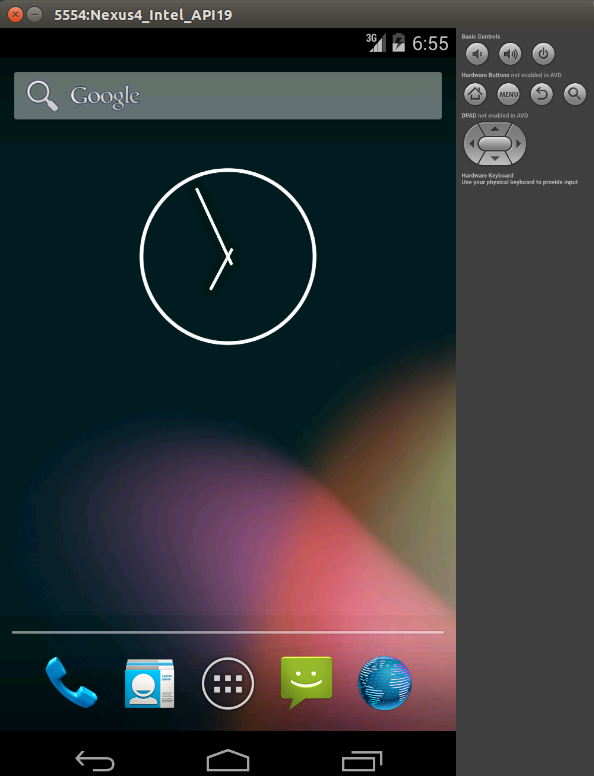
\includegraphics[keepaspectratio, scale=0.3]{Media/Captures/emulator_api_19.png}
      \caption{Emulador Android API 19}
      \label{fig:android_emulator19}
    \end{figure} 
    
    De esta manera podemos probar la aplicación, que será lanzada en el emulador/dispositivo una vez termine su instalación. \\[.2cm]

	\textbf{2 - Teniendo un emulador previamente lanzado (ver sección anterior para ver cómo se lanza) o un dispositivo móvil ya conectado por USB:} \\[.2cm]
	
	En este caso es todavía más sencillo el proceso de construcción. Nos vamos a la carpeta raíz del proyecto  y podemos compilar e instalar la aplicación con un solo comando:

 	 \begin{lstlisting}[style=console, numbers=none]
		$ ant debug install
	\end{lstlisting}	
 	 
 	 Es importante destacar que este comando solo funciona si tenemos un único emulador o dispositivo conectado, de lo contrario habrá que utilizar el método anterior. \\[.2cm]

    
    \subsubsection{Proceso de Depuración} \label{sssec:debug}
    
    Una vez instalada una aplicación, podemos depurar su código en ejecución usando la herramienta DDMS del ADT en conjunto con la vista de Debug de Eclipse. Pero antes hay que especificar qué aplicación queremos depurar de las que puedan estar instaladas en el dispositivo o emulador. \\[.2cm]

En el caso del emulador debemos lanzar la aplicación llamada “Dev Tools” y abrir el menú “Developer Options”. Dentro de este menú habilitaremos las opciones de “USB debugging” y de  “Wait for debugger”. Además pulsaremos sobre “Select Debug app” y seleccionaremos la aplicación que queremos depurar. \\[.2cm]

En el caso de un dispositivo Android debemos ir a los Ajustes del dispositivo y seleccionar el menú de Opciones de Desarrollador. Aquí habilitamos las opciones de "Depuración de USB"  (si no esta habilitada ya) y de "Esperar al depurador". Además pulsamos donde pone "Seleccione una aplicación para depurar" y elegimos la aplicación que queremos depurar. \\[.2cm]

Una vez hecho esto, cada vez que ejecutemos la aplicacion saldrá un mensaje de advertencia y se quedará esperando a que conectemos un depurador para continuar con su ejecución. Para esto, nos vamos a Eclipse y abrimos la vista de DDMS. Aquí nos aparecerá, entre otras cosas, un espacio con todos los procesos en ejecución en el dispositivo/emulador. Localizamos el proceso de nuestra aplicación y pulsamos sobre el bichillo verde para conectar el depurador a ella. Llegados a este punto la aplicacion continua su ejecución en el emulador y aparece un escarabajo verde al lado del proceso de la app en la ventana de DDMS, que indica que se esta depurando ese proceso. Es entonces cuando podemos abrir la vista de depuración de Eclipse y proceder a trabajar con breakpoints para depurar y estudiar el código con el fin de solucionar errores.

    
  \subsection{Migración: Identificación y Solución de Problemas}
  
	  El objetivo de esta parte del proyecto es conseguir que el cliente de SwellRT se pueda desplegar en Android para asi conseguir que se conecte al servidor WIAB que tambien incluye. Para ello lo primero que haremos será desplegar el servidor en nuestro ordenador clonando el repositorio de GitHub de SwellRT y siguiendo los pasos descritos en el Readme del proyecto \cite{ref:swellRT_github}. Para comprobar que el servidor se ha instalado correctamente, podemos ejecutarlo por consola (ver Readme) y abrir un navegador web con la dirección http://localhost:9898. Si nos aparece una ventana de Login de WIAB es que ya tenemos un servidor WIAB corriendo en nuestro ordenador. Creamos entonces un usuario y contraseña de prueba. Este paso es importante ya que la aplicación Android intentará conectarse contra este servidor mientras estemos haciendo pruebas de desarrollo. \\[.2cm]
	  
	  A continuación crearemos un proyecto Android en Eclipse e incluiremos en él todas las clases de SwellRT. Uno de los componentes principales de Android a la hora de desarrollar son las \textbf{Actividades} \cite{ref:android_activities}, que representan las pantallas que se le muestran al usuario y que responden a su interacción programáticamente. Por tanto, crearemos una nueva actividad  
	  principal (waveAndroid.java) que se ejecutará al lanzar la aplicación y que por el momento intentará conectarse al servidor especificando por código el usuario y contraseña que hemos creado antes en el servidor. Wave realiza este login contra el servidor usando dos tecnologias: HTTP \cite{ref:http_authentication} y WebSockets \cite{ref:webSocket_ref}.
	  
  
    \subsubsection{Conexion HTTP}
	
	Wave fue desarrollado para utilizar el protocolo WebSocket para la conexión al servidor, pero esta tecnología necesita realizar una autenticación HTTP previa. Lo primero que haremos será otorgar \textbf{permisos de conexión a internet} a nuestra aplicación. Android utiliza un \textbf{sistema de permisos} \cite{ref:android_permissions} para controlar los privilegios de cada aplicación. Estos permisos se declaran en el \textbf{Manifiesto} de la aplicación \cite{ref:android_manifest}, archivo que declara sus características. Para ello basta con añadir lo siguiente al manifest.xml de la aplicación:
	  
	  \lstset{language=XML, breaklines=true, autogobble=true, basicstyle=\ttfamily\footnotesize}
	  \begin{lstlisting}[frame=single]
	  	<uses-permission android:name="android.permission.INTERNET"/>
	  \end{lstlisting}
	  
	  	 Tambien hay que tener en cuenta que cuando nos encontramos en el emulador no estamos en la misma red que el ordenador en el que trabajamos, por lo que la conexion a la URL http://localhost:9898 no es valida. No obstante, esto tiene facil solucion pues \textbf{el emulador de Android define unas direcciones IP de red especiales} \cite{ref:android_netAddress} para este tipo de casos. Basta con sustituir localhost por la direccion 10.0.2.2 para conseguir acceder al servidor WIAB desplegado en el ordenador. La direccion URL sera por tanto: \textbf{http://10.0.2.2:9898}. 
	  
	 Lo siguiente que haremos será ejecutar el código de Login del cliente SwellRT para intentar localizar dónde se lleva a cabo la conexion HTTP. Para ello llamamos desde la actividad principal (WaveAndroid.java) al método startSession() de la clase WaveClient.java pasándole el usuario y la contraseña antes creados.
 
	 Esto provoca un error de ejecución y la aplicación se cierra. Lo siguiente que hacemos es depurar la aplicación (Ver Seccion \ref{sssec:debug}) estudiando el LogCat \cite{ref:android_logcat} (Ver Figura \ref{fig:android_logcat}) para ver donde se produce el error. Descubrimos que el problema estaba localizado en el método login() de la misma clase, que intentaba realizar una \textbf{peticion POST HTTP} al servidor utilizando un \textbf{RequestBuilder} de la libreria \textbf{com.google.gwt.http.client}. He aquí el primer problema: la actual conexión utiliza métodos de GWT/Javascript para hacer la petición post y Android no es compatible con esta tecnología.   
	 
	\begin{figure}[H]
      \centering
	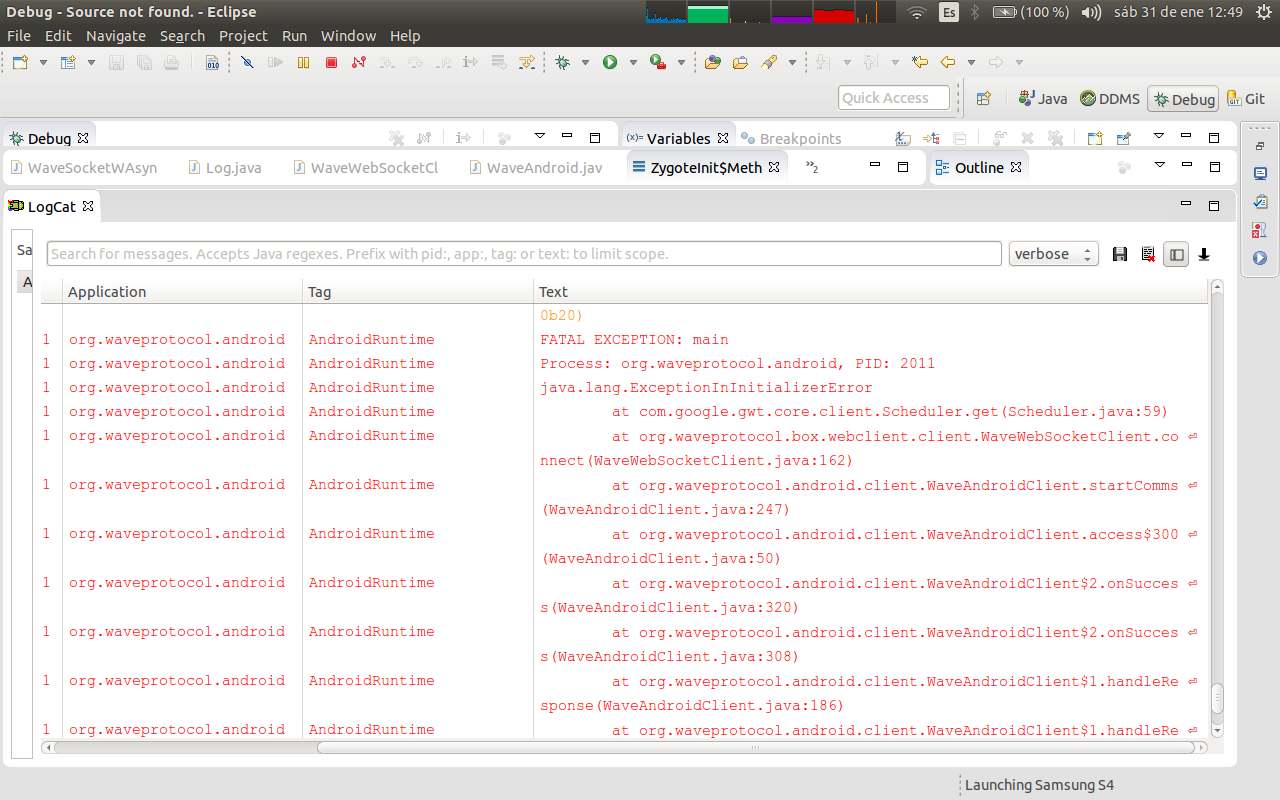
\includegraphics[keepaspectratio, scale=0.3]{Media/Captures/logcat_example.png}
      \caption{Ejemplo de Traza de Error en Logcat}
      \label{fig:android_logcat}
    \end{figure} 
	 
	 Hay por tanto que encontrar una librería similar compatible con Android que construya una peticion \textbf{HTTP POST} y la envie al servidor. La primera opcion que valoramos fue utilizar la \textbf{libreria HTTP Apache} \cite{ref:apache_http}, incluida en el SDK de Android desde sus primeras versiones. Sin embargo, Google recomienda \cite{ref:http_recommmendations} a partir del API 10 (Android 2.3 "Gingerbread") utilizar la \textbf{libreria HttpURLConnection} \cite{ref:android_httpUrlConnection}. Por tanto esta ultima es la que elegimos para la migracion. \\[.2cm] 
	 
	 De forma simplificada, este seria un esquema de la nueva estructura del login HTTP:
	 
	  \lstset{language=Java, breaklines=true, autogobble=true, basicstyle=\ttfamily\footnotesize, commentstyle=\color{OliveGreen}, keywordstyle=\color{MidnightBlue}}
	  \begin{lstlisting}[frame=single]	  
import java.net.HttpURLConnection;

private void login(final String user, final String password, final Callback<String, String> callback) {
  
		//Construct the URL String urlStr with the server, user and password parameters
  
	    URL url = new URL(urlStr); //String 
	    HttpURLConnection connection = (HttpURLConnection) url.openConnection(); //Open the connection to the given URL

	    connection.setDoOutput(true); // allow the POST connection
	    connection.setRequestProperty("Accept-Charset", CHARSET);
	    connection.setRequestProperty("Content-Type", "application/x-www-form-urlencoded;charset="
		+ CHARSET);

	    OutputStream out = connection.getOutputStream(); 
	    out.write(queryStr.getBytes(CHARSET)); //Set the POST parameters

	    if (connection.getResponseCode() != 200) {
		      //ERROR during the connection
		      connection.disconnect(); //Disconnect from the server.
	    } else {
		      //Continue with the login process (WebSocket)
		      connection.disconnect(); //Disconnect from the server.
	    }		      
}	    
	  \end{lstlisting}  
	  
	  Sin embargo, aquí no acaba el problema. Por cuestiones de usabilidad y de respuesta a la interacción del usuario, Android establece dos reglas para trabajar con el proceso de la actividad que se le esta mostrando al usuario (llamado \textbf{UI Thread}) \cite{ref:android_processes}:
	  
	  \begin{itemize}
	  	\item \textbf{1. No bloquear el UI Thread}
	  	\item \textbf{2. No acceder al UI Thread directamente desde otro Thread}
	  \end{itemize}
	  
	  La conexión a un servidor es un proceso susceptible de durar un tiempo variable según las condiciones de la red, lo cual deja la aplicación en espera hasta que se realiza dicha conexión,  bloqueando el UI Thread. Por tanto, decidimos usar un hilo (Thread) por separado en forma de \textbf{AsyncTask} \cite{ref:android:asynctask} para llevar a cabo la tarea de Login, tal y como recomienda Google hacer para trabajar con conexiones a la red \cite{ref:android_networking}. La ventaja por tanto de usar otro hilo para esto es que la actividad principal no se bloquea. \\[.2cm]
	  	 
	  El siguiente es un esquema del AsyncTask encargado del Login: \\[.2cm]
	  
	  \lstset{language=Java, breaklines=true, autogobble=true, basicstyle=\ttfamily\footnotesize, commentstyle=\color{OliveGreen}, keywordstyle=\color{MidnightBlue}}
	  \begin{lstlisting}[frame=single]	  
private class LoginTask extends AsyncTask<String, Void, String> {

    @Override
    protected String doInBackground(String... params) { //method that executes on the new Thread without blocking the UI Thread
      login(params[0], params[1], params[2]); //Do the login     
    }

    @Override
    protected void onPostExecute(String result) { //method that executes on the UI Thread once doInBackground() finishes its execution.
    
      if (result != null) { 
        callback.onLogin(); //Notify the login success using the proper callback method
      } else { //The doInBackGround method has had a problem and the result of its execution was null
        callback.onError("Wave Login Error"); //Notify the login error using the proper callback method
      }
    }
}    
	  \end{lstlisting} 
	  
	  Es importante tambien destacar que la arquitectura de SwellRT y de Wave esta planteada de manera que utiliza llamadas asíncronas (callbacks) para notificar al resto de la aplicacion del resultado de los procesos de conexión al servidor.
	    
\textbf{Llegados a este punto, tenemos un proceso de login Http que hace uso de la libreria HttpUrlConnection y de un AsyncTask para realizar esa primera conexión al servidor.} Depuramos la aplicación y comprobamos que efectivamente el login Http se realiza correctamente (la respuesta del servidor tiene código 200). \textbf{Sin embargo la aplicacion aun no funciona correctamente, pues se cierra al intentar ejecutar el código que se encarga del siguiente paso del login: la conexión por WebSocket.}    
    
    \subsubsection{Conexion WebSocket}
    
    
    
    
    \subsubsection{Login}
  
  \subsection{Organización y Resultados}
    \subsubsection{Servicio Android}
    \subsubsection{Resultado de la Migracion}
    \subsubsection{Diagramas y Dependencias}
\newpage
\thispagestyle{sectioned}
\chapter{Creación de aplicación Android (AppName)}

\section{Introducción}
Una vez que habíamos elegido la tecnología que soportaría el núcleo de nuestra aplicación, teníamos que decir que implementación le íbamos a dar a nuestra aplicación móvil. Para ello teníamos que tener en cuenta las características que nos ofrecía Wave:

Edición colaborativa.

Tiempo real.

Consistencia.

Después de darle unas cuantas vueltas de las posibles implementaciones que podríamos realizar sobre estas características potenciales, decidimos realizar una sesión de brain storming. En esta sesión aparecieron temas tan dispersos como wikis colaborativas, aplicaciones con inteligencia artificial, aportaciones colaborativas en política, edición de vídeos y música, cursos de formación colaborativos, etcétera.

	\begin{figure}[H]
      \centering
	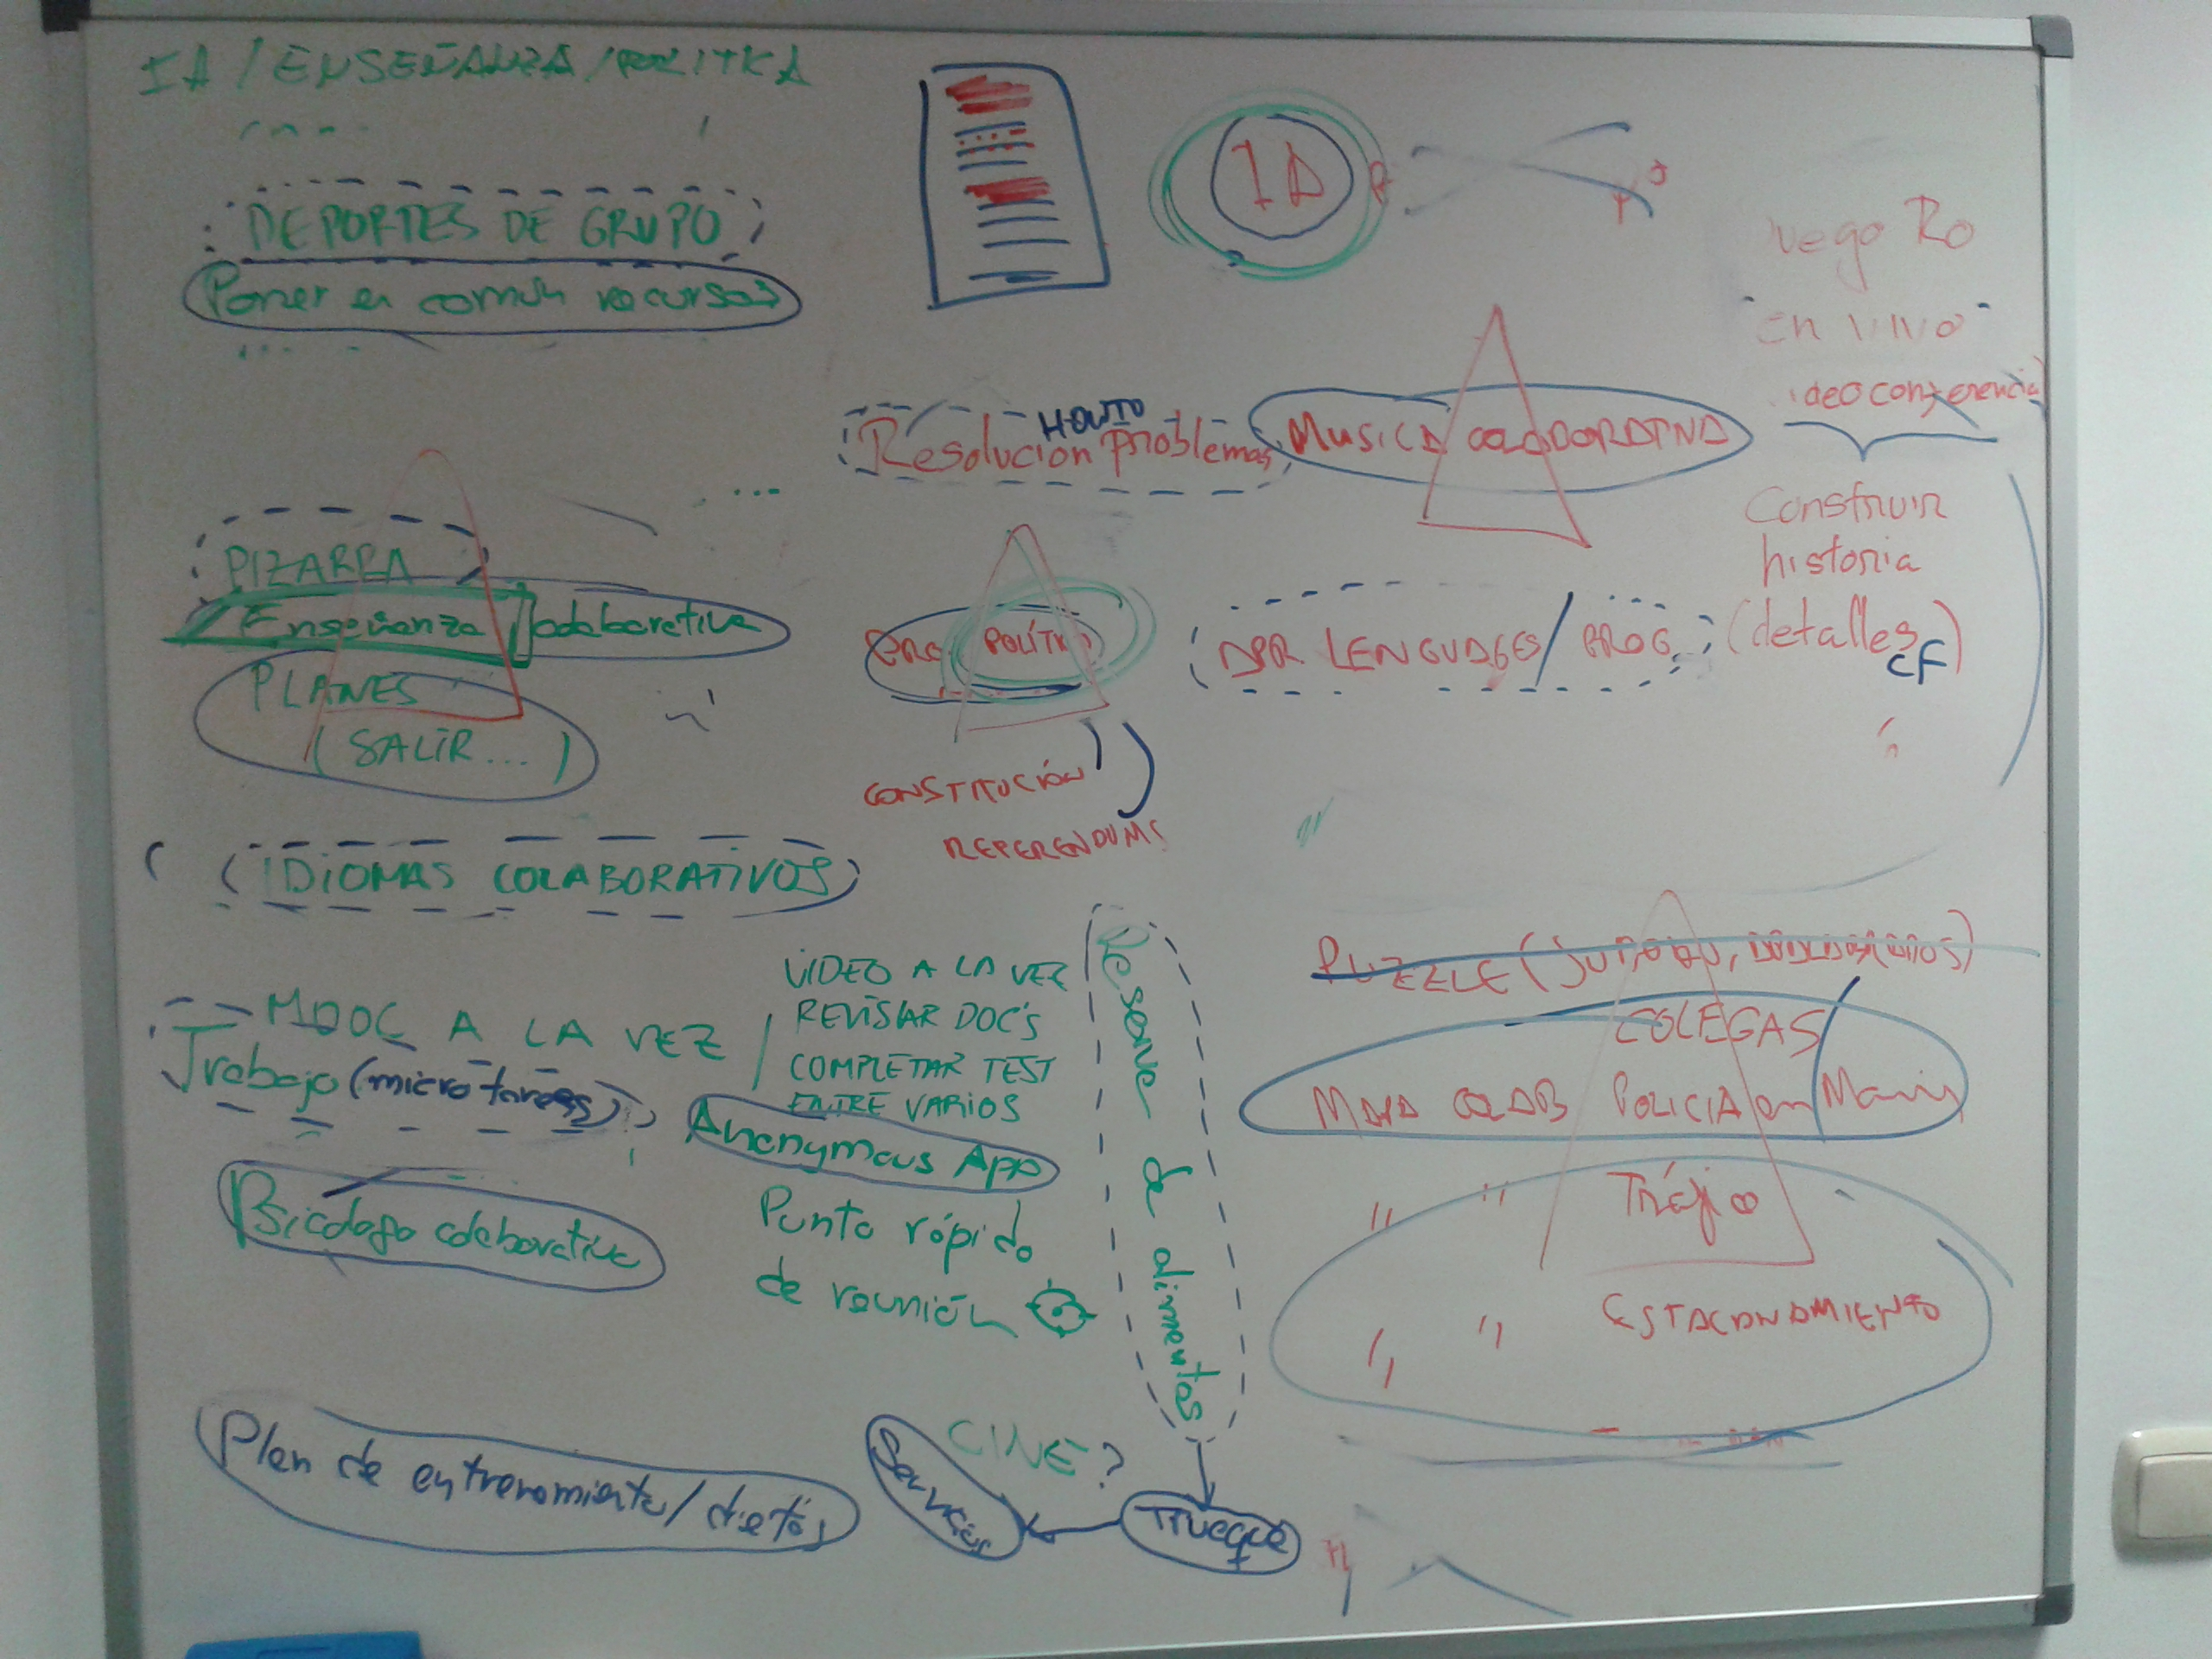
\includegraphics[keepaspectratio, scale=0.15]{Media/Captures/brainstorming.jpg}
      \caption{Brainstorming sobre la idea a desarrollar}
      \label{fig:brainstorming}
    \end{figure}
    
Con un gran repertorio de ideas expuestas sobre la sesión, descartamos aquellas que no nos motivaban llevarlas a cabo. Por lo que nos quedamos con tres ideas fundamentales a desarrollar en nuestra aplicación: Política, Música, Inteligencia Artificial y Mapas. Surgieron varias ideas colaborativas como desarrollar documentos políticos, programas electorales, comunicación entre colectivos en tiempo real, aprendizaje de música, edición de partituras y obras, aplicaciones colaborativas con inteligencia artificial, edición de mapas en tiempo real, lexicalización, etcétera.

Finalmente debido a intereses comunes, decimos realizar una aplicación colaborativa relacionado con el mundo de la política. Con el objetivo de que pudiera tener cierta repercusión y utilidad en las próximas citas electorales durante el año 2015. En esta aplicación podríamos recurrir a la edición de contenidos en tiempo real, ya fueran propuestas políticas, programas electorales y otro tipo de documentos. Como también hacer uso de alguna herramienta de Inteligencia Artificial para automatizar algunas tareas o realizar recomendaciones sociales.

\subsection{Adentrándonos en la idea}
La idea a desarrollar generada en una época dónde la política parecía haber despertado el interés de una parte considerable de la ciudadanía, podría ser una herramienta útil para participar en temas políticos que forma sencilla y atractiva. Dejando atrás los tópicos yo no entiendo de política, la política es aburrida, no sé a quién votar o no he leído nunca un programa electoral entre otros.

La herramienta ofrecería una nueva forma de participar en la política y de llevar a los ciudadanos los programas electorales ofertados por las diferentes formaciones políticas. De tal forma que los ciudadanos pudieran leer aquellos puntos de los programas más leídos, debatidos, comentados, etcétera. Así cualquier usuario tendría todos programas electorales en su bolsillo, por lo que no tendría que ir a la página web de cada formación política y descargarse un documento de 200 páginas. Pensamos que esta forma de presentar un programa político en un mundo donde las posibilidades de  comunicarnos se han desarrollado exponencialmente, no era la mejor manera de llegar a la mayor parte de la ciudadanía.

Por otra parte, la aplicación también debería ofrecer alguna herramienta donde realizar propuestas y debatirlas entre todos. De tal forma que tanto la ciudadanía como las formaciones políticas pudieran saber en cualquier momento cuáles son las principales preocupaciones de los ciudadanos y qué medidas o soluciones proponen para resolverlas.

Desde un primer punto de vista subjetivo, la aplicación quedó dividida en dos partes. Por un lado tendríamos los programas políticos que presentaran las formaciones políticas. Y por otro, todas las propuestas que elaboraran los ciudadanos individualmente o en colectivos sociales.

\subsection{Política en el mundo de la Informática}

\subsection{Democracia}

	\subsubsection{Democracia representativa}
	
	\subsubsection{Democracia participativa}
	
	\subsubsection{Democracia directa}
	
	\subsubsection{Democracia deliberativa}
	

\section{1ª Parte: Programas Políticos}
En esta sección se desarrollará en profundidad todo lo relacionado con los partidos políticos.

  \subsection{Estado del Arte}
En la actualidad no existe ningún tipo de aplicación orientada a debatir los programas electorales de los partidos políticos. Concretamente no hay ningún tipo de plataforma que agrupe los programas electorales de las diferentes candidaturas.
Lo más parecido que hemos podido encontrar han sido aplicaciones elaboradas por un partido político, orientada a dar a conocer su candidatura. En ella podremos ver la candidatura, vídeos y el programa electoral entre otros. Por ello pasamos a analizar las aplicaciones encontradas:

	\subsubsection{UPyD Parla}
La aplicación que presenta el candidato de UpyD Carlos Alt Bustelo para la alcaldía de Parla. Se trata de una alicación divulgativa donde podemos conocer todo lo esencial de la candidatura de UpyD para las elecciones del municiono de Parla en Mayo de 2015. Los candidatos, el programa, vídeos, etcétera.

	\begin{figure}[H]
      \centering
	
\includegraphics[keepaspectratio, scale=0.35]{Media/Captures/UPyDParla.png}
      \caption{UPyD Parla}
      \label{fig:upydparla}
    \end{figure}

	\subsubsection{$\sharp$RecuperaCórdoba}
De forma similar a la anterior, la candidatura de Pedro García a la provincia de Córdoba de Izquierda Unida, presenta su propuesta de gobierno de forma compacta. En la aplicación podremos encontrar la lista de los candidatos propuestos a la comunidad cordobesa, el programa electoral de la formación, las propuestas del partido, noticias de última hora y vídeos.

	\begin{figure}[H]
      \centering
	
\includegraphics[keepaspectratio, scale=0.35]{Media/Captures/IURecuperaCordoba.png}
      \caption{$\sharp$RecuperaCórdoba}
      \label{fig:recuperacordoba}
    \end{figure}
    
    	\subsubsection{PP Canarias}
    	
La delegación del Partido Popular en Canarias, presenta su aplicación móvil para promocionar a sus candidatos para las elecciones autonómicas y municipales de Mayo de 2015. La aplicación nos avisará de los eventos electorales, podremos consultar los candidatos, novedades, galería de imágenes y por su puesto el programa electoral.

	\begin{figure}[H]
      \centering
	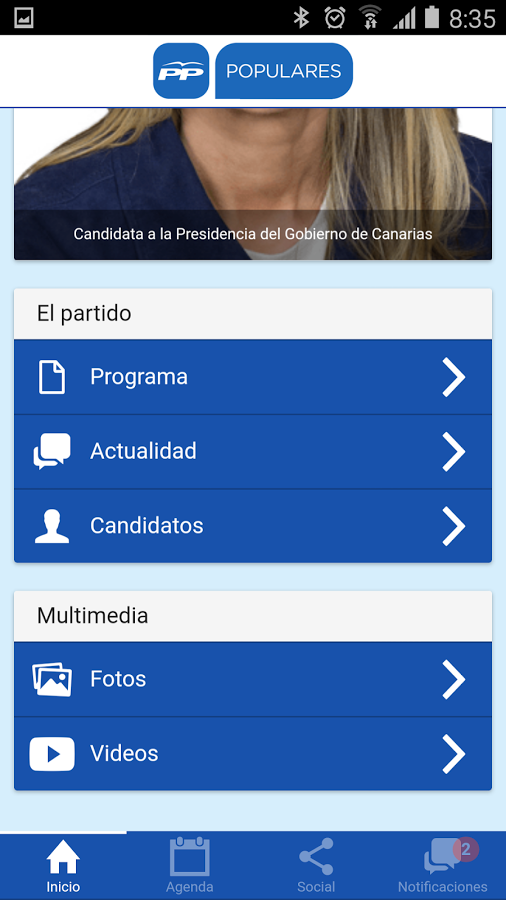
\includegraphics[keepaspectratio, scale=0.35]{Media/Captures/ppcanarias.png}
      \caption{PP Canarias}
      \label{fig:ppcanarias}
    \end{figure}

	\subsection{Intención}

La intención fundamental de la aplicación es llevar los programas electorales a los bolsillos de los ciudadanos. Vivimos en una sociedad digital, donde cada vez son más las personas que utilizan los teléfonos inteligentes para realizar todo tipo de tareas en su vida cotidiana.

En los últimos años las diferentes formaciones políticas han subido sus programas electorales a un documento en formato pdf que estaba disponible en su página web. Este documento generalmente extenso, no es un medio fácil de divulgar y mostrar a la ciudadanía. Por ello pensamos que una aplicación que pudiera visualizar las principales secciones de los programas políticos, podría ser especialmente útil para acercar los programas a los electores.

Llegando a crear un espacio donde poder informase sobre las distintas ofertas electorales, debatir las propuestas que propone cada formación política reducido en una aplicación que podremos consultar en cualquier momento.
  
	\subsection{Objetivos}
	
La aplicación pretende llevar las principales partes de los programas electorales de los partidos que se presenten a las elecciones. Por tanto, cualquier usuario podrá visualizar el apartado que desee consultar de cualquier partido político. Siendo esta la forma menos amigable de leerlo, se utilizarán distintas formas para compartir o divulgar determinadas secciones más populares.

Al inicio de la aplcación, mostrará una lista de las secciones de los programas más valoradas, más debatidas, peor valoradas e incluso las más incomprendidas. Por tanto creemos que puede ser una forma de acercar aquellas secciones más populares de forma más eficaz, al contrario que tener que consultar una determinada página dentro de un extenso pdf.

	\begin{figure}[H]
      \centering
	
\includegraphics[keepaspectratio, scale=0.5]{Media/Captures/captTopSections.png}
      \caption{Vista principal de secciones}
      \label{fig:captTopSections}
    \end{figure}
    
Dentro de cada sección podemos visualizar el contenido de la sección a la que referencia el programa, y tendremos la opción de valorarla de forma positiva o negativa. También añadimos la posibilidad de indicar que no se ha entendido la sección. Pues a la hora de leer una propuesta de gobierno ubicada en una sección del programa, bien nos puede gustar, disgustar o simplemente no haber entendido la idea y por ello no votarla de forma positiva o negativa.

	\begin{figure}[H]
      \centering
	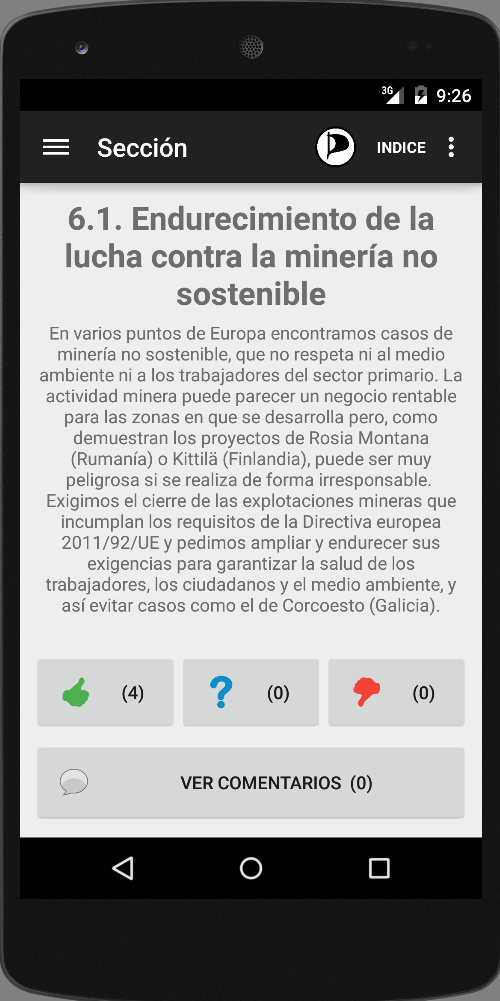
\includegraphics[keepaspectratio, scale=0.5]{Media/Captures/section.png}
      \caption{Visualizando una sección}
      \label{fig:captSection}
    \end{figure}
    
Sin olvidarnos de la parte social, en cada sección podemos hacer comentarios para intentar debatir las ideas fundamentales que propone la sección. O incluso hacer referencia a una determinada frase o párrafo.
	\subsection{Usabilidad}
	
	\subsection{Revisión de la aplicación}
Una vez que habíamos implementado todos los objetivos fundamentales de la aplicación, decidimos hacer una revisión para poner a prueba la aplicación. Para ello nos reunimos con un grupo de Labodemo \cite{ref:labodemo}, responsables del desarrollo de los portales de participación ciudadana del partido político Podemos \cite{ref:podemos} y la candidatura ciudadana de unidad popular Ahora Madrid \cite{ref:ahoramadrid}.

	\subsubsection{Reunión con Labodemo}
Tuvimos la oportunidad de establecer una conversación con dos miembros de Labodemo, en la que aprovechamos la oportunidad de mostrarles la aplicación que estábamos desarrollando. Ambos tenían experiencia en el desarrollo de plataformas de participación ciudadana en internet y nuevas tecnologías. Además fueron los responsables del desarrollo de los portales de participación del partido político Podemos y la candidatura ciudadana de unidad popular Ahora Madrid.

Limitarnos a mostrar las diferentes secciones de cada programa les resultó útil. Aunque no suficiente como para atraer a una cantidad considerable de usuarios. Antes de hablar con ellos, habíamos planteado desarrollar propuestas colaborativas en tiempo real aprovechando Wave. Pero no comprendieron la libertad de dar al usuarios la creación de propuestas colaborativas en tiempo real.

Dándole una vuelta al desarrollo de las propuestas de la aplicación, nos sugirieron que para atraer a usuarios a utilizar nuestra aplicación, deberíamos dejar cierta libertad a colectivos sociales. Por ejemplo, un grupo de animalistas debería tener un “espacio” en la aplicación donde poder crear sus propias propuestas, e incluso hacer comparativas personalizadas de lo que proponen los diferentes programas sobre los animales. Así surgirían propuestas y comparativas divididas por colectivos que abarcarían diferentes temáticas. Un usuario poco activo podría buscar un colectivo de profesores porque resulta ser su profesión, y ver las propuestas que se llevan a cabo o visualizar una comparativa respecto las medidas de educación de los diferentes programas políticos.

Organizar estas propuestas no sería tarea sencilla. En un principio se propuso como diferentes temas que puede tener un foro, en forma de post. Más tarde llegamos a la conclusión de que sería más cómodo para los colectivos dar la libertad de crear sus propios hilos, y en cada uno de ellos publicar las propuestas relacionadas con su colectivo.

Por último insistieron mucho en el tema de las comparativas. Sería de gran utilidad que la aplicación tuviera una parte de comparativas en la que los usuarios pudieran comparar los programas políticos en vez de leerlos sección por sección. Resultaría de gran interés a un autónomo visualizar las medidas que proponen los diferentes partidos políticos para los autónomos. Pero estas comparativas no podría realizarlas cualquiera, por lo que deberían realizarlas periodistas o expertos que hubieran realizado algún tipo de comparativa similar anteriormente. Nos sugirieron contactar con periodistas o colectivos que hubieran publicado algún tipo de comparativa en cuando a programas o medidas, para obtener algún tipo de ayuda o consejo a seguir.
	
	\subsubsection{Conclusión}

La reunión con dos de los miembros de Labodemo resultó de gran interés. Pues desde que decidimos la idea que íbamos a implementar, nunca habíamos puesto en práctica la aplicación o al menos no la habíamos verificado con el “mundo real”.

Los integrantes de Labodemo eran expertos en desarrollo de portales de participación ciudadana. Y sobre todo estaban muy familiarizados con el uso común que les suele dar la gente a este tipo de aplicación. Por lo que sabían determinar las claves para que una aplicación tuviera un movimiento considerable de usuarios desde el comienzo.

El tema de visualizar los programas políticos no les gustó demasiado. Expusieron que un ciudadano de a pie, no iba a molestarse en leer los programas políticos. Bien porque no los entienda o porque les resulte aburridos. Ellos argumentaban que los colectivos sociales serían los usuarios más activos en nuestra aplicación, por lo que debíamos enfocar más el desarrollo hacia la partición ciudadana y el uso de propuestas o comparativas por colectivo.

Tras esta reunión decidimos replantear la aplicación en base a los consejos que obtuvimos con la reunión de Labodemo. Incluimos las propuestas como parte de nuestra aplicación y empezamos a pensar la forma de colaborar de grupos y colectivos. También intentamos contactar con colectivos y personas interesadas en el desarrollo de la aplicación. Finalmente, conseguimos concretar una entrevista con Javier de la Cueva \cite{ref:jdelacueva}.
	
	\subsubsection{Reunión con Javier de la Cueva}
	
	\subsubsection{Conclusión}

  
\section{2ª Parte: Propuestas y Categorización}
  \subsection{Estado del Arte}

  \subsection{Intención}
  \subsection{Objetivos}
  \subsection{Usabilidad}
  
\section{3ª Parte: Encuestas de intención de voto}
  \subsection{Estado del Arte}

  \subsection{Intención}
  \subsection{Objetivos}
  \subsection{Usabilidad}
  
  
\section{Tecnologias y Metodologías de la app}

  \subsection{Arquitectura de la aplicacción}
  
La arquitectura está compuesta por tres módulos principales de los que hablaremos en profundidad en las siguientes subsecciones. Como cliente móvil tendremos la aplicación desarrollada en Android, que realizará peticiones HTTP al servicio web alojado en OpenShift, una plataforma que permite alojar servicios web de forma gratuita. Dentro del servicio contaremos con una API RESTful que será quien gestione las peticiones de la aplicación móvil mediante el protocolo HTTP.

	\begin{figure}[H]
      \centering
	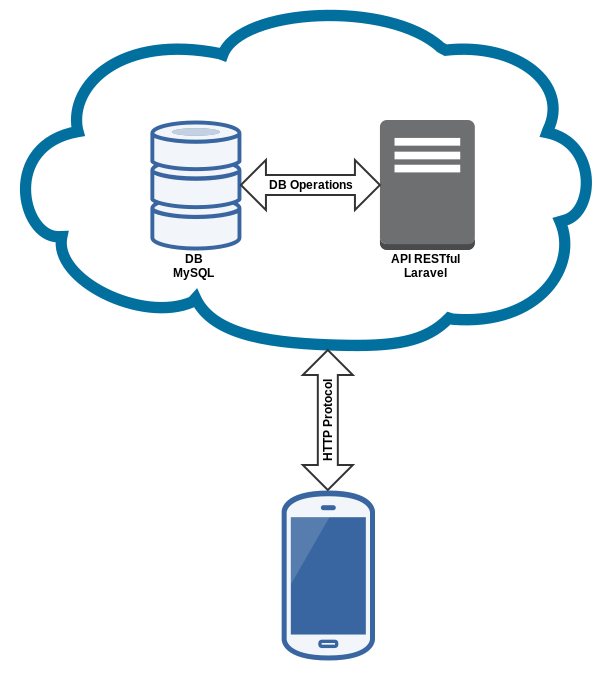
\includegraphics[keepaspectratio, scale=0.4]{Media/Captures/architecture.png}
      \caption{Arquitectura de la aplicacción.}
      \label{fig:architecture}
    \end{figure}

Por último, la base de datos MySQL alojada en el servidor de OpenShift \cite{ref:OpenShift}, almacenará toda la información relacionada con la aplicación. La API RESTful será quien gestione las operaciones de la base de datos.

	\subsection{Back-end}

  		\subsubsection{Base de Datos}\label{sssec:database}
Para la implementación de la base de datos, se ha utilizado un modelo relacional para la definición de las tablas. Utilizando MySQL \cite{ref:MySQL} como sistema de gestión de base de datos phpMyAdmin \cite{ref:phpMyAdmin} como herramienta de gestión gráfica de la base de datos.

La base de datos está formada por un total de 12 tablas donde se almacena toda la información relacionada con los programas de los partidos políticos, las propuestas ciudadanas, encuestas, comparativas, …, y otros datos más técnicos como la gestión de los usuarios, la relación de los comentarios o la relación entre las secciones y comparativas entre otras.

	\begin{figure}[H]
      \centering
	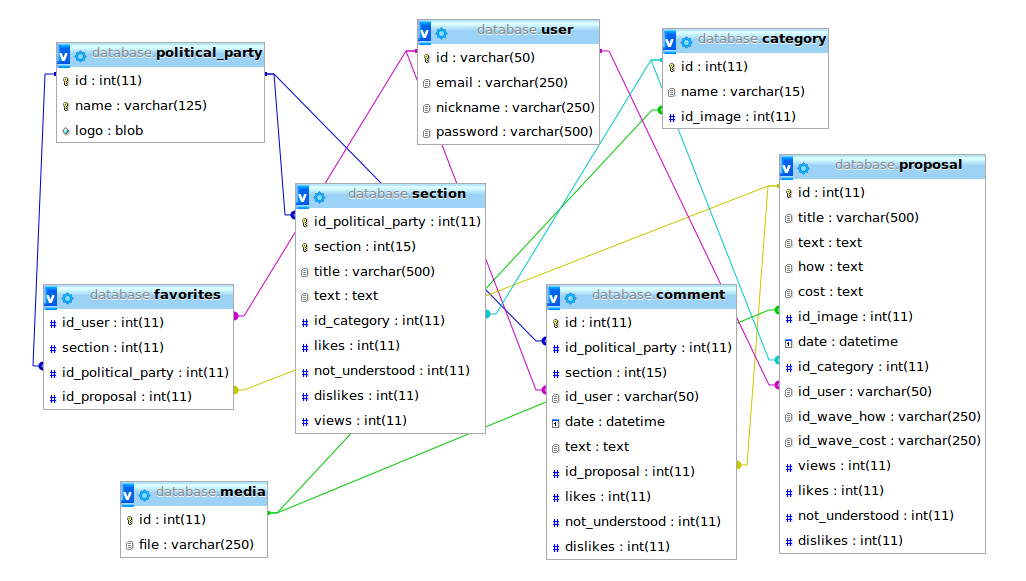
\includegraphics[keepaspectratio, scale=0.30]{Media/Captures/database.png}
      \caption{Modelo entidad-relación de la base de datos.}
      \label{fig:ermodel}
    \end{figure}
    
Las tablas section y \textit{political-party} son utilizadas para guardar información estática en la aplicación. Es decir, en la tabla \textit{political-party} se almacenan los partidos políticos que se presentan a unas elecciones, y en la tabla \textit{section}, las diferentes secciones de un programa electoral. Tan sólo modificaremos las columnas de \textit{likes}, \textit{dislikes}, \textit{not-understood} y \textit{views} para obtener estadísticas de uso de cada sección. El resto de las columnas permanecerán intactas.

Las demás tablas serán utilizadas para guardar datos dinámicos en la aplicación. Datos que normalmente genera un usuario visitando una sección de un programa, creando una propusta, haciendo un comentario, etc.

    
		\subsubsection{Service REST}\label{sssec:rest}
		
Para establecer la conexión de la base de datos con la aplicación desarrollada en Android, hemos utilizado Laravel como servicio web. Laravel \cite{ref:laravel}  un framework de código abierto para desarrollar aplicaciones web con PHP 5.

Laravel nos permite montar un sistema de RESTful para que el cliente móvil pueda hacer peticiones al servicio web. Estas peticiones se realizan mediante el protocolo HTTP, en función de la operación que deseemos hacer, haremos una petición GET, POST, PUT, …, etcétera.

	\begin{figure}[H]
      \centering
	
\includegraphics[keepaspectratio, scale=0.30]{Media/Captures/laravel5.png}
      \caption{Pantalla principal de Laravel 5.}
      \label{fig:laravel5}
    \end{figure}

Establecer un servicio RESTful nos proporciona una gran flexibilidad. Pues no solo podremos hacer peticiones desde el cliente en Android, si no que más adelante si pretendemos desarrollar una versión web o incluso un cliente para iOS, las peticiones serán las mismas.

Para organizar las diferentes peticiones en función de su uso y requisitos, Laravel permite montar una API REST (Representational State Transfer), un estilo de arquitectura software para sistemas hipermedia distribuidos como la World Wide Web. Este término se originó en una tesis doctoral sobre la web escrita por Roy Fielding \cite{ref:RESTPhd}.

  \subsection{Frontend}

\newpage
\thispagestyle{sectioned}
\chapter{Resultados y Conclusiones}

\section{Discusion de Resultados}
%\addcontentsline{toc}{chapter}{\numberline{Global Results}}

\section{Conclusiones}
%\addcontentsline{toc}{chapter}{\numberline{Conclusion}}



\newpage
\thispagestyle{sectioned}
\pagenumbering{arabic}
\chapter{Trabajo a Futuro}

\section{Mejoras}

\addcontentsline{toc}{chapter}{\numberline{}Bibliography}

\rhead{}
\renewcommand{\headrulewidth}{0pt}

\bibliographystyle{unsrt}
\bibliography{bibliography}

\end{document}
